\section{Implementation}

\subsection{Simulated data sources}
\label{sec:sources}
\textbf{Streaming source.} The file \code{fleet\_model.py} is a small agent-based model. Each vehicle is a
state machine: \emph{offline} $\rightarrow$ \emph{idle} $\rightarrow$ \emph{enroute} to a pickup
$\rightarrow$ \emph{on\_trip} $\rightarrow$ \emph{idle}. Drivers work fixed shifts, and two drivers work at
night so that data never stops. Ride requests arrive at random, and the rate depends on the zone type (city
centre, commercial, residential) and on the hour of the day, with morning and evening peaks. Road speed is
slower in Colombo rush hours. Fares follow simple LKR rules for tuk-tuks, mini cars and cars, with a surge
at peak hours for cars. Every real second each online vehicle sends one ping, and trip start and trip end
events are sent at the moment they happen.

\textbf{Daily-batch source.} At every simulated midnight the model writes a ground-truth file with the true
kilometres of each vehicle. After a random partner delay, \code{batch\_producer.py} turns it into the cost
file: fuel = kilometres divided by fuel efficiency, times the fuel price of the day, and maintenance = daily
upkeep, plus wear per kilometre, plus a service bill on some days. The file is written to a temporary name
and then renamed, so a reader never sees half a file. A manifest with the row count and a SHA-256 checksum is
written last.

Five vehicles have special profiles. These are the stories the pipeline must find without being told:
\begin{itemize}
\item \textbf{V007} (\emph{degrading}): fuel use rises by 15\% and garage time by 2.5 hours every day.
\item \textbf{V013} (\emph{high maintenance}): double upkeep and a service bill on about one day in three.
\item \textbf{V026} (\emph{fuel anomaly}): the partner reports 30 to 40\% more kilometres and fuel than the GPS shows.
\item \textbf{V021} and \textbf{V027} (\emph{idle prone}): the drivers take long breaks and wait a lot.
\end{itemize}

\subsection{Speed layer}
The speed layer is one Spark application (\code{speed\_layer.py}) with the four streaming queries in
Table~\ref{tab:queries}. Each query has its own checkpoint, so after a crash it continues from the exact
Kafka offsets where it stopped.

\begin{table}[!htb]
\centering\small
\caption{Streaming queries of the speed layer.}
\label{tab:queries}
\begin{tabularx}{\textwidth}{@{}P{2.4cm} L P{3.5cm} P{1.1cm}@{}}
\toprule
\textbf{Query} & \textbf{Main operations} & \textbf{Output} & \textbf{Trigger} \\
\midrule
\code{raw\_archive} & copy every record with its Kafka partition, offset and time & Parquet master dataset & 30 s \\
\code{zone\_hourly} & parse, validate, 10-minute watermark, de-duplicate by \code{event\_id}, zone lookup, 1-hour tumbling windows by zone & \code{speed.zone\_hourly} & 10 s \\
\code{vehicle\_daily} & same cleaning, 1-day windows by vehicle (fares and kilometres so far) & \code{speed.vehicle\_daily} & 10 s \\
\code{vehicle\_state} & latest position and status of each vehicle, idle streaks, idle alerts, invalid events & \code{speed.vehicle\_state}, alerts, dead-letter topic & 5 s \\
\bottomrule
\end{tabularx}
\end{table}

\textbf{Cleaning.} Nine validation rules check each event, for example a missing id, a GPS point outside
Sri Lanka, a negative speed or a trip end without a fare. Invalid events go to the dead-letter topic and to
the \code{ops.dead\_letters} table with the list of broken rules. Repeated events are removed with
\code{dropDuplicates\allowbreak Within\allowbreak Watermark} on \code{event\_id}.

\textbf{Enrichment.} GPS points become zone names through a stream-static broadcast join with a small
lookup grid of 0.005-degree cells. Fares count in the zone where the trip started.

\textbf{Late data.} The watermark trails the newest event time by 10 simulated minutes (5 real seconds).
A window stays open until the watermark passes its end, so a late event is still counted if its hour is
open. An event that arrives after its window has closed is dropped, and Spark reports how many. This keeps
the state small. The batch layer later counts these events correctly.

\textbf{Exactly-once writes.} Spark's \code{foreachBatch} can run a micro-batch again after a failure. Each
batch therefore starts its PostgreSQL transaction by inserting its (query name, batch id) pair into
\code{ops.speed\_batches}. If the pair already exists, the batch was committed before and is skipped. The
ledger row and the data rows are committed together, so each micro-batch is applied exactly once.

\textbf{Idle alerts.} For every vehicle we keep \code{idle\_since}, the start of its idle streak. One alert
opens after 90 idle simulated minutes and closes when the vehicle takes a ride or goes offline.

\subsection{Batch layer and orchestration}
\label{sec:batch}
The Airflow DAG \code{fleet\_daily\_batch} (Figure~\ref{fig:dag}) runs once per simulated day. Its steps are:
\begin{enumerate}[itemsep=1pt]
\item \textbf{resolve\_target\_day} picks the oldest day without batch results, or the day given as a
parameter for a rerun.
\item \textbf{wait\_for\_expense\_file} is a sensor. After 1.5 simulated days without a file it fails and
raises an alert.
\item \textbf{validate\_expense\_file} checks the SHA-256 checksum, header and row count against the
manifest, and copies the file into the master dataset.
\item \textbf{wait\_for\_raw\_telemetry} waits until two simulated hours after midnight, so late events of
the day are archived.
\item \textbf{spark\_batch\_recompute} runs \code{spark-submit batch\_layer.py} for the day.
\item \textbf{data\_quality\_checks} tests the published numbers, for example that less than 5\% of events
were invalid.
\item \textbf{build\_daily\_report} writes the HTML and CSV report, and \textbf{purge\_speed\_layer} deletes
speed-layer rows for days that the batch layer now owns.
\end{enumerate}

\begin{figure}[!htb]
\centering
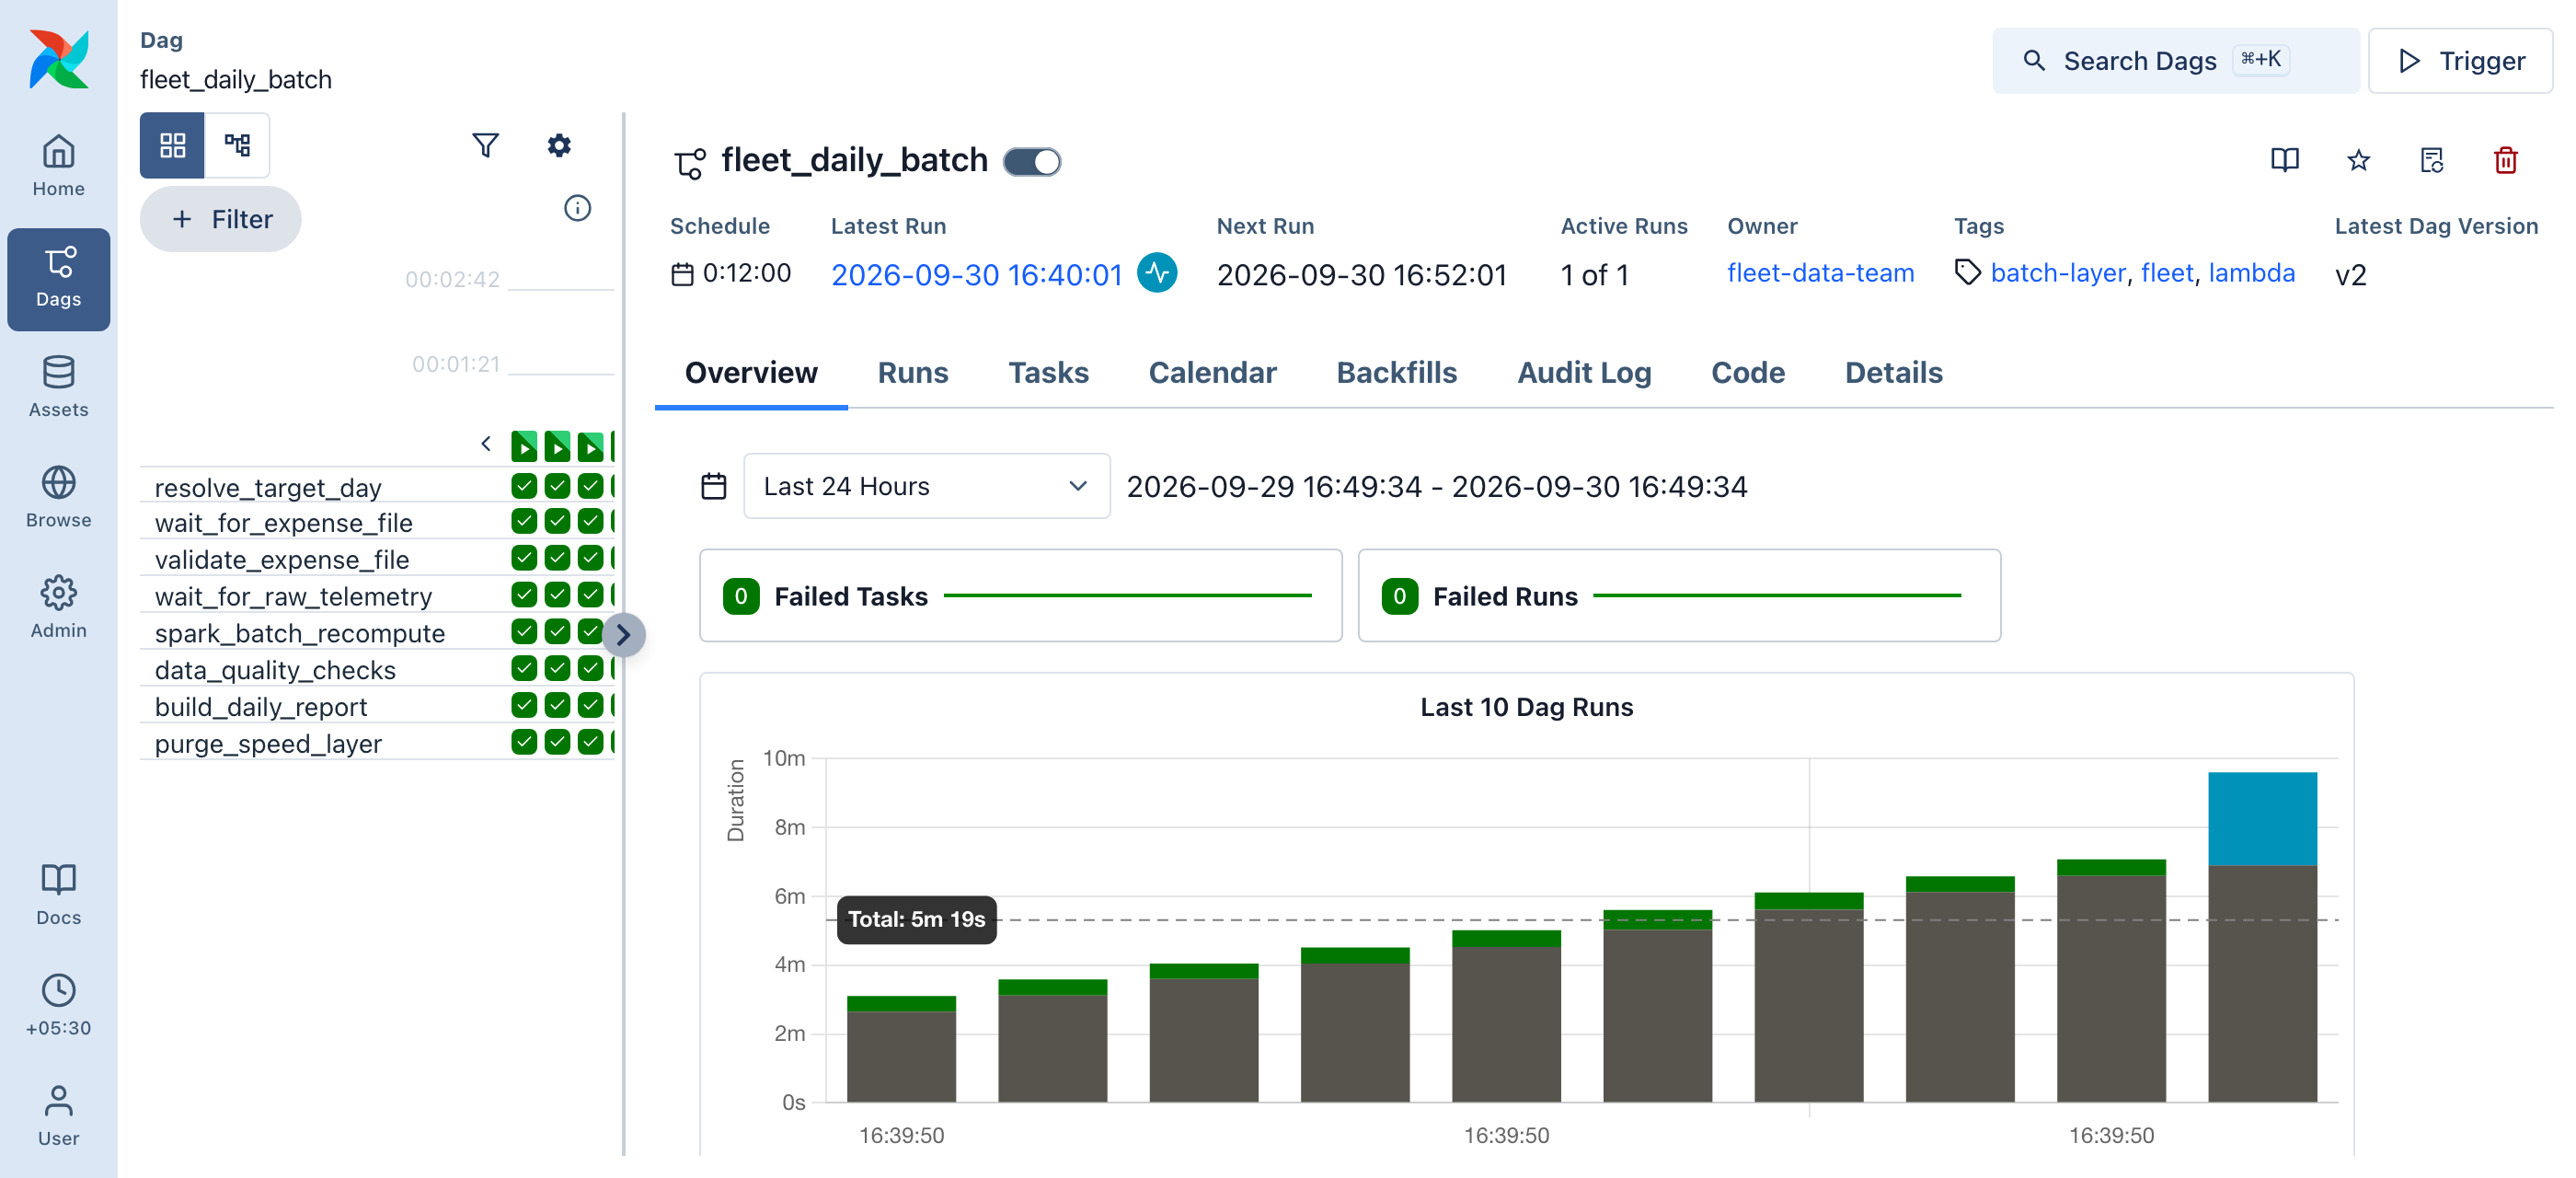
\includegraphics[width=0.85\textwidth]{figures/airflow_grid.png}
\caption{Airflow view of the DAG \code{fleet\_daily\_batch}. Each row is a task and each column is one run,
that is one simulated day. Green means success.}
\label{fig:dag}
\end{figure}

The Spark batch job reads only the master dataset. It removes invalid and repeated events over the whole
day, counts late events, and uses window functions on each vehicle's pings in time order to measure minutes
on a trip, minutes idle and the longest idle streak. It checks every cost row (numbers, dates, known
vehicles, repeated records). Bad rows go to a quarantine table with a reason. Then it joins the day's
telemetry with the costs. The profit of a vehicle for one day is:
\[
\text{net profit} = \text{fares} - 0.30 \times \text{fares} - \text{fuel cost} - \text{maintenance cost}
\]
A vehicle is \emph{unprofitable} when its net profit is below zero and \emph{at risk} when its margin is below
15\%. It is \emph{becoming unprofitable} when it is unprofitable or at risk and its profit fell on two days
in a row, or when it was profitable yesterday and loses money today. Days with a garage service bill are
never counted, because one large bill is not a trend. The job also
writes plain-English reasons, such as ``high fuel cost'' or ``reported km differ from GPS by 32\%''. All
views of the day are replaced in one PostgreSQL transaction, so users never see half a day.

\subsection{Serving layer}
\label{sec:serving}
The serving layer has three parts. The \textbf{FastAPI service} offers the endpoints in
Table~\ref{tab:api} and a \code{/docs} page. \textbf{Grafana} has three provisioned dashboards: live fleet
operations, daily profitability and pipeline health. The \textbf{daily report} is an HTML page (with a CSV
file) for fleet managers.

\begin{table}[!htb]
\centering\small
\caption{Main API endpoints.}
\label{tab:api}
\begin{tabularx}{\textwidth}{@{}P{5.9cm} L@{}}
\toprule
\textbf{Endpoint} & \textbf{Answer} \\
\midrule
\code{/api/v1/fleet/realtime} & live fleet status, trips and fares today, fares by zone \\
\code{/api/v1/zones/hourly?date=} & zone by hour metrics (batch view for finished days, speed view for today) \\
\code{/api/v1/profitability/live} & profit projected for today from live fares and batch cost rates \\
\code{/api/v1/profitability/daily?date=} & exact profit of every vehicle for a finished day \\
\code{/api/v1/alerts} & idle alerts and pipeline alert notifications \\
\code{/api/v1/pipeline/status} & freshness of each layer, recent runs and dead letters \\
\code{/reports/\{date\}.html} & the daily report \\
\bottomrule
\end{tabularx}
\end{table}

The most important Lambda merge is the \textbf{live profit projection}. The speed layer knows today's fares
and kilometres, and the batch layer knows each vehicle's recent fuel cost per kilometre and maintenance per
day. The view \code{serving.v\_vehicle\_profit\_live} combines them to show which vehicles are losing money
\emph{today}, before today's cost file exists. This answers the second part of the business question during
the day, and the batch layer confirms it with exact numbers after midnight.
